\documentclass[a4paper,12pt]{article} % тип документа

% report, book



%  Русский язык

\usepackage[T2A]{fontenc}			% кодировка
\usepackage[utf8]{inputenc}			% кодировка исходного текста
\usepackage[english,russian]{babel}	% локализация и переносы
\usepackage{graphicx}
\graphicspath{{./}}
\DeclareGraphicsExtensions{.png,.jpg}


% Математика
\usepackage{amsmath,amsfonts,amssymb,amsthm,mathtools} 


\usepackage{wasysym}

%Заговолок
\author{Бредихин Александр}
\title{Домашняя работа №4}



\begin{document} % начало документа

\maketitle

\subsection*{Задача 1}
Составим рекуренту по написанному в условие задачи алгоритму, 
$$
\left\{\begin{array}{l}
T(n)=T\left(\left[\frac{n}{4}\right]\right)+1+T\left(\left[\frac{n}{4}\right]\right)+2020+T\left(\left[\frac{n}{4}\right]\right), n>2020 \\
T(n)=O(1), n \leq 2020
\end{array}\right.
$$
Решаем полученную рекуренту, $ T(n)=3 \cdot T\left(\left[\frac{n}{4}\right]\right)+O(1) $ с помощью дерева вызовов:
\begin{center}
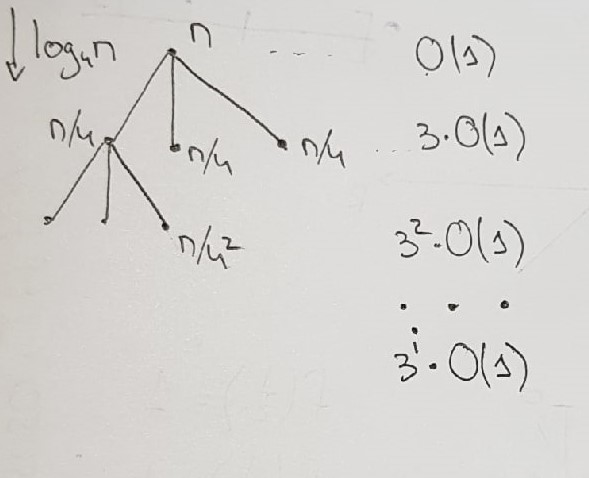
\includegraphics[width=0.7\textwidth]{tree_1}
\end{center}
Глубина дерева: $ \log_{4}n $, так как при каждом шаге происходит деление на 4. Количество слов, напичатанное алгоритмом вычисляется суммой: 
$$
\sum_{i=0}^{\log n} O(1) \cdot 3^{i}=O(1) \cdot\left(1+3+3^{2}+\ldots+3^{\log_{4} n}\right)=O(1) \cdot \frac{3^{\log _{4} n+1}-1}{2}=\theta\left(n^{\log _{4} 3}\right)
$$
Ответ: $ \theta\left(n^{\log _{4} 3}\right) = \theta(n)  $

\subsection*{Задача 2}
Докажем по индукции, что алгоритм всегда останавливается и  все числа будут равными НОДу элементов массива.\\

База индукции: для $ n = 2 $ -- выполнено (алгоритм Евклида)\\

Предположение индукции: пусть выполнено для $ n $ чисел\\

Шаг индукции: Добавляем в массив ещё одно число (их становится $ n+1 $, если НОД элементов после этого не изменился, то применяем предположение индукции для первых $ n $ элементов, а затем из последнего вычитаем любой из них, так как НОД всех чисел не изменился, то через конечное число вычитаний получим его. Если после добавления, НОД всех чисел изменился, то применяем наше предположение для первых $ n $ и затем последних $ n $ чисел, получаем, что все числа будут сведены к общему НОДу\\



\subsection*{Задача 3}
Задача: предположим, удалось установить, что любое число можно возвести в квадрат за $O(n)$, где $n$ -- длина числа в двоичной записи. Докажите, что тогда любые два числа можно перемножать за $O(n)$, где $n$ -- длина максимального из чисел в двоичной записи.\\

Произведение двух чисел $ b $ и $ c $, можно находить следующим образом:
\begin{equation} \label{formula_3}
(b+c)^{2}=b^{2}+c^{2}+2 b c \rightarrow b c=\frac{(b+c)^{2}-b^{2}-c^{2}}{2}
\end{equation}
Заметим, что сумма чисел $ b+c $ выполняется, за $O(n)$, где $ n $ -- длина наибольшего из чисел и в результате получим число не более $ n+1 $ бита (побитовое суммирование) (аналогично с вычитанием). Так как у нас есть алгоритм возведения числа в квадрат, за $O(n)$, то операции: $b^{2}, \quad c^{2}, \quad (b+c)^{2}$ будут работать за $O(n)$. Деление на 2 -- удаление последнего бита: $O(1)$. \\
Из формулы \eqref{formula_3} получаем, что перемножение двух чисел производится за $O(n)$ , где $ n $ -- длина наибольшего из чисел.


\subsection*{Задача 4}
Из свойств НОД и НОК получаем формулу: 
$$
a \cdot b = \text{НОД}(a,b) \cdot \text{НОК}(a,b) \longrightarrow 
\text{НОК}(a,b) = \frac{a \cdot b}{\text{НОД}(a,b)}  
$$
Пусть максимальная битовая запись числа имеет длину $ n $. Используем обычный алгоритм Евклида, для нахождения $ \text{НОД}(a,b) $ -- выполняется за $ O(\log n) $, делим одно из чисел на полученный НОД (побитовое деление), а затем умножаем на другое (побитовое умножение). В худшем случае эти арифметические операции выполняются за $ O(n^2) $. Получается, общая сложность этого алгоритма: $ O(n^2) $




\subsection*{Задача 5}
Для решения каждого из пунктов пользуемся мастер-теоремой решения рекурент вида: $T(n)=a \cdot T\left(\frac{n}{b}\right)+f(n)$\\
{\bf a)} 
$$
\begin{aligned}
&T(n)=36 \cdot T\left(\frac{n}{6}\right)+n^{2}\\
&\log _{b} a=\log _{6} 36=2
\end{aligned}
$$
$ \longrightarrow $ 2ой случай, так как $ n^2 = f(n) = \Theta(n^2) $, по основной теореме:\\
Ответ: $ T(n) = \Theta(n^2 \log n) $\\
{\bf b)}
$$
\begin{aligned}
&T(n)=3 \cdot T\left(\frac{n}{3}\right)+n^{2}\\
&\log _{b} a=\log _{3} 3=1
\end{aligned}
$$
$ \longrightarrow $ третий случай, так как:
$$
\begin{aligned}
&1) \quad \exists \varepsilon=1: f(n)=n^{2}=\Omega\left(n^{1+1}\right)=\Omega\left(n^{2}\right) - \text{верно} \\
&2) \quad \exists c=\frac{1}{2} \in(0,1): 
3 \cdot \left(\frac{n}{3}\right)^{2} \leq c \cdot n^{2} 
\quad 1 \leq 3 c=3 \cdot \frac{1}{2} - \text{верно}
\end{aligned}
$$
$ \Longrightarrow $ по основной теореме:\\
Ответ: $ T(n) = \Theta(n^2) $\\
{\bf c)}
$$
\begin{aligned}
&T(n)=4 \cdot T\left(\frac{n}{2}\right)+\frac{n}{\log n}\\
&\log _{b} a=\log _{2} 4=2\\
&\longrightarrow \text{1ый случай, так как:} \quad \exists \varepsilon=1: \frac{n}{\log n}=O(n) \\
& \text{так как} \quad \exists c = 1, \exists N = \text{основание логарифма} : \forall n \geq N \rightarrow \frac{1}{\log n} \leq 1
\end{aligned}
$$
$ \Longrightarrow $ по основной теореме:\\
Ответ: $ T(n) = \Theta(n^2) $\\

\subsection*{Задача 6}
Задача: на вход подаётся числовой массив $A$ из $n$ элементов. Требуется найти число инверсий -- $ inver $ в массиве, т.\,е. пар индексов $(i,j)$, таких что $i<j$ и $a[i] > a[j]$.\\
Предложим рекурсивный алгоритм, аналогичный сортировке слиянием, то есть есть функция $ number\_inversions $, которая получает на вход массив $ a $ и возвращает количество инверсий в нём, а массив $ a $ становится отсортированным по возрастанию.\\
Заметим, что в массиве размером 1, число инверсий равно 0, а он сам является отсортированным (База индукции)\\
На каждом шаге разбиваем исходный массив на 2 части пополам. Вызываем нашу функцию $ number \_ inversions $ от каждой из частей. Первый вызов вернёт $ inver\_1 $ -- количество инверсий в левом подмассиве, $ inver\_2 $ -- в правом и подмассивы станут отсортированными.\\

Ищем все инверсии, которые возникают при <<склеивании>>  двух подмассивов, так как $ i<j $(индексы левого подмассива точно меньше, чем индексы правого), нужно искать для каждого элемента отсортированного правого подмассива, сколько элементов в левом больше него (получим, что для $ i<j $ и $ a[i] > a[j] $) и прибавлять в переменную $ count $, тогда возвращаемое число инверсий будет равно $ inver = inver\_1+inver\_2+count $\\
$ count $  ищем следующим способом: уснавливаем 2 указателя: $ index\_1  $ и $ index\_2 $ на концы каждого из подмассивов $ a\_1 $ и $ a\_2 $  ($ A $ -- исходный массив, $ index $ -- указатель, устанновленный на конец массива $ A $). 
\begin{itemize}
\item если: $\quad a\_1[index\_1] > a\_2[index\_2] $\\
$ \Rightarrow A[index] = a\_1[index\_1] $ \\
$ count += index\_2 + 1$ \\
$ index -- ; \quad index\_1 --$\\
(если текущий элемент в левом подмассиве больше, чем текущий элемент в правом, то он больше всех остальных в правом. А их количество как раз равно  $ index\_2 + 1$)
\item если $\quad a\_1[index\_1] < a\_2[index\_2] $ \\
$ \Rightarrow A[index] = a\_2[index\_2] $ \\
$ index -- ; \quad index\_2 --$
\item если $\quad a\_1[index\_1] == a\_2[index\_2] $ \\
$ \Rightarrow A[index] = a\_2[index\_2] \quad index--; \quad index\_2--;$ \\
$ count += index\_2 $ \\
$A[index] = a\_1[index\_1]$ \\
$ index -- ; \quad index\_1 --$ \\
(если текущие элементы равны то сначала в массив $ A $, кладём значение элемента из правого подмассива и уменьшаем соответствующий ему индекс, а затем увеличиваем количество инверсий, так как $ a[i] > a[j] $ -- строгий знак)
\end{itemize}
Возвращаемое значение учитывает количество инверсий и в левом и в правом подмассивах, поэтому их исходный порядок не важен для всех элементов из правого подмассива выполнено, что его индекс больше, чем индекс любого из левого, поэтому количество инверсий на текущем шаге считается правильно. (Шаг индукции)\\

Корректность алгоритма доказана по индукции (рекурсивный алгоритм). Сложность -- $\mathcal{O}(n\log{}n)$, делаем то же самое, что и в сортировке слияния плюс арифметические операции на каждом шаге, сложность которых $\mathcal{O}(1)$

\subsection*{Задача 7}
Задача: Докажите, что если $T_1(n) = aT_1(\frac{n}{b})+ f(n)$,\; $T_2(n) = aT_2(\frac{n}{b})+ g(n)$ и $f(n) = \Theta(g(n))$, то $T_1(n) = \Theta(T_2(n))$.

$\square$ Рекуренты вида: $T(n) = aT(\frac{n}{b})+ F(n)$ с помощью дерева вызова раскрываются следующим образом (на $ k $ом уровне сумма имеет вид: $a^kF(\frac{n}{b^k})$): 
\begin{equation} \label{recur}
T(n) = aT(\frac{n}{b})+ F(n) = C \sum_{k=0}^{\log n} a^{k} F\left(\frac{n}{b^k}\right)
\end{equation}
По определению $\Theta$оценки:
$$
f(n)=\theta(g(n)) \Longleftrightarrow \exists c_{1,2}: \exists N: \forall n \geq N \rightarrow c_1 g(n)\leqslant f(n) \leqslant c_{2} g(n)
$$
Из этого и того что $T_1(n) = aT_1(\frac{n}{b})+ f(n)$,$ \quad $ $ \forall n \geq N $ выполняется:
$$
a T_{1}\left(\frac{n}{b}\right)+c_1 g(n) \leq T_{1}(n) \leq a T_{1}\left(\frac{n}{b}\right)+c_{2} g(n)
$$
Пользуяся для этого утверждения уравнением \eqref{recur} и тем, чему равны исходные рекуренты $ T_1 $ и $ T_2 $, получаем:
$$
C_1\sum_{n=0}^{\log n} a^{i} g\left(\frac{n}{b^i}\right) \leq T_{1}(n) \leq C_{2} \sum_{n=0}^{\log n} a^{i} g\left(\frac{n}{b^{i}}\right)
$$
$$
\frac{C_{1}}{C} T_{2}(n) \leq T_{1}(n) \leq \frac{C_{2}}{C} T_{2}(n) $$
А это и есть определение $ \Theta $ оценки, значит: $T_{1}(n)=\theta\left(T_{2}(n)\right)$.
\begin{flushright}
	$\blacksquare$
\end{flushright}



\subsection*{Задача 8}

{\bf a)} $T(n)=3 T\left(\left[\frac{n}{4}\right]\right)+T\left(\left[\frac{n}{6}\right]\right)+n$ \\
Построим дерево вызовов:
\begin{center}
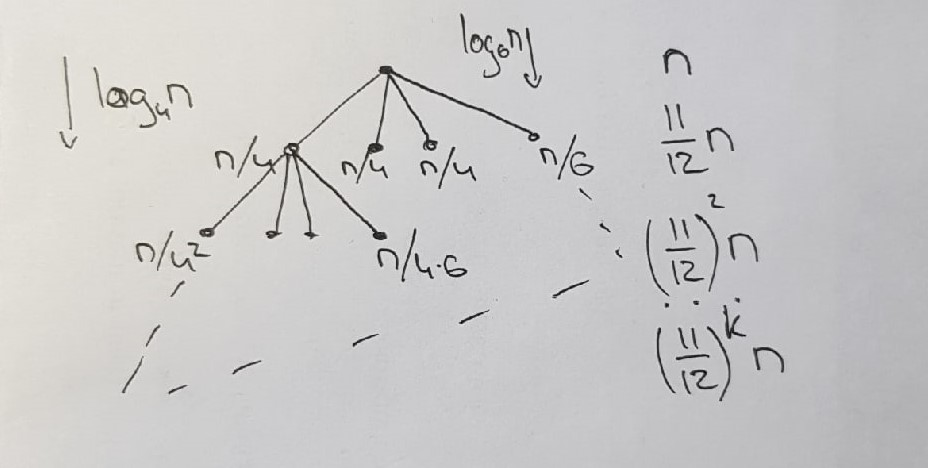
\includegraphics[width=0.7\textwidth]{tree_81}
\end{center}
Заметим, что сумма операций на $ k $ой строчке равняется: $ \left(\frac{11}{12}\right)^{k} n $, глубина дерева: минимальная (каждый раз делим на 6) равняется $ \log_6n $, максимальная (каждый раз делим на 4) -- $ \log_4n $. При достаточно больших $ n $ можно считать, что дерево <<ровное>> (от основания логарифма не зависит). Тогда количество операций, которые делает рекурента оценивается суммой:
$$
\sum_{k=0}^{\log n}\left(\frac{11}{12}\right)^{k} n=n \cdot \frac{\left(\frac{11}{12}\right)^{\log n}-1}{\frac{11}{12}-1}=12n\left(1-\left(\frac{11}{12}\right)^{\log n}\right)
$$ 
При больших $ n $: $ \lim\limits _{n \rightarrow \infty}\left(1-\left(\frac{11}{12}\right)^{n}\right) \rightarrow 1 $, следовательно, $ T(n)=C \cdot n=\theta(n) $\\
Ответ: $ T(n) = \theta(n) $\\

{\bf b)} $T(n) = T(\alpha \cdot n) + T((1-\alpha)\cdot n) + \Theta(n)$\\
Делаем аналогично предыдущему пункту, строим дерево вызовов: 
\begin{center}
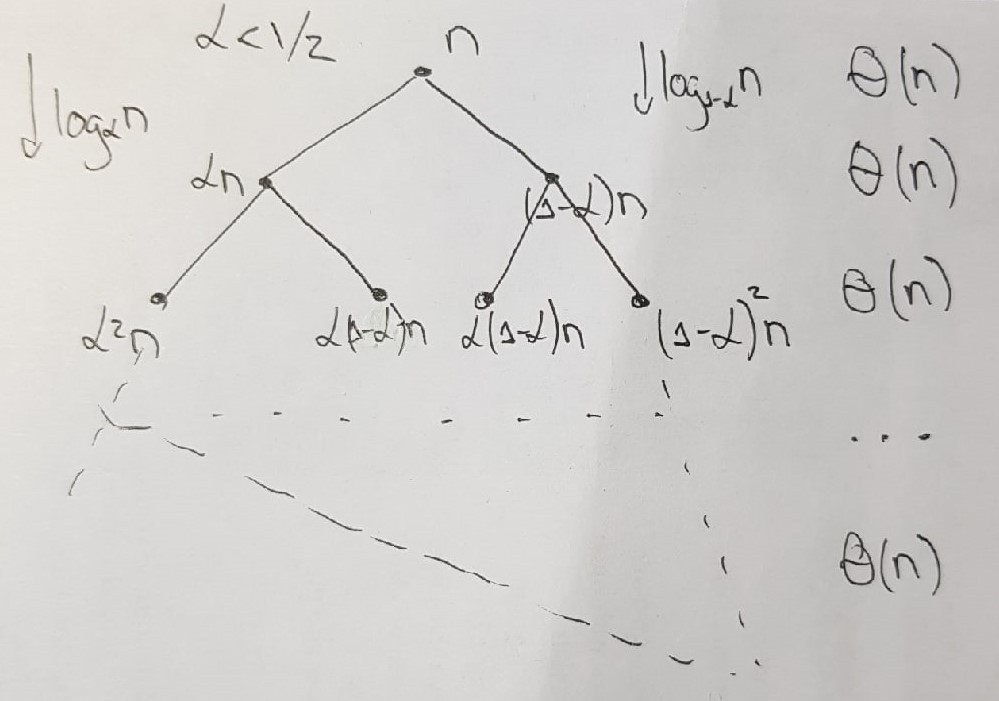
\includegraphics[width=0.7\textwidth]{tree_82}
\end{center}
Без ограничения общности возьмём $ \alpha < \frac{1}{2} $. Заметим, что сумма операций на каждом уровне дерева, равна $ \theta(n) $ (так как бином Ньютона: для квадрата $ (1)^{2}=(\alpha+1-\alpha)^{2}=\alpha^{2}+2 \alpha(1-\alpha)+(1-\alpha)^{2} $, аналогично для больших степеней). Глубину веток деревьев оцениваем аналогично предыдущему пункту: $\log_{\alpha }n $ -- минимальная (так как $ \alpha < \frac{1}{2} $) и максимальная -- $\log_{(1 - \alpha)}n$. \\
Получается: $ \log_{\alpha}n \cdot \Theta(n) \leqslant T(n) \leqslant  \log_{(1 - \alpha)}n \cdot \Theta(n) $\\
При больших $ n $ основание логарифма не влияется на асимптотику, следовательно, $T(n) = \Theta(n \cdot logn)$\\
Ответ: $T(n) = \Theta(n \cdot logn)$\\

{\bf c)} $T(n)=T(\lfloor n/2\rfloor)+2\cdot T(\lfloor n/4\rfloor)+\Theta(n)$	\\
Аналогично предыдущим пунктам строим дерево вызовов: 
\begin{center}
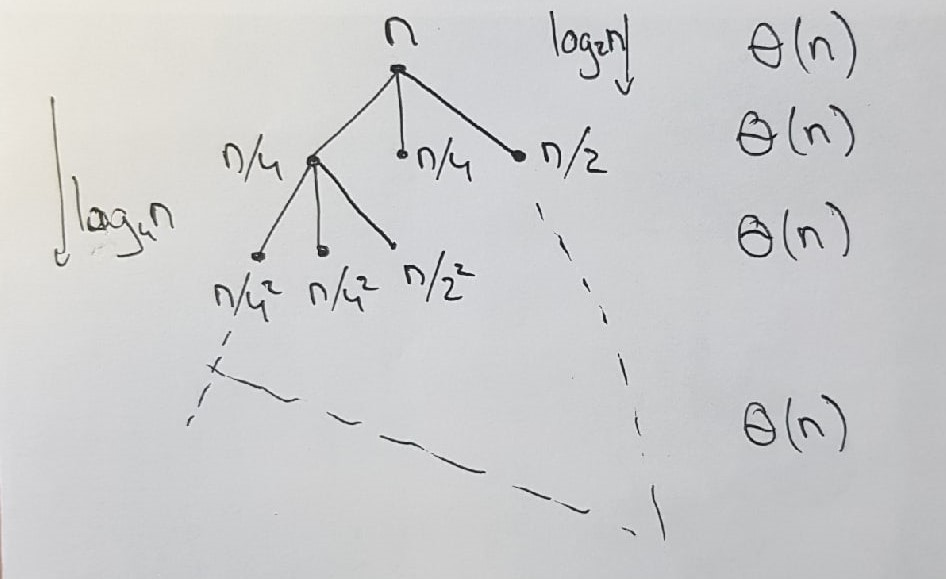
\includegraphics[width=0.7\textwidth]{tree_83}
\end{center}
На каждом уровне дерева рекурента выполняется одинаковое количество действий, равное $ \theta(n) $ (снова бином Ньютона). Длина самой длинной ветки дерева равна $\log_2(n)$, а самой короткой -- $\log_4(n)$. Получается: $\log_{4}n \cdot \Theta(n) \leqslant T(n) \leqslant  \log_{2}n \cdot \Theta(n) $. При больших $ n $ основание логарифма можно пренебречь, поэтому $ T(n) = \Theta(n \cdot logn) $\\
Ответ: $ T(n) = \Theta(nlogn) $

{\bf d)} $T(n) = 27T(\frac{n}{3})+\frac{n^3}{\log^2 n} $\\
Используем основную теорему: $ \log_b a= log_3 27 = 3 $. Покажем, что будет выполняться 1ый пункт, то есть 
$$
\exists \varepsilon>0: f(n)=\frac{n^{3}}{\log ^{2} n}=O\left(n^{3-\varepsilon}\right)
$$
Найдём формулу для $ \varepsilon $:
$$
\frac{n^{3}}{\log ^{2} n} \leq C \cdot \frac{n^{3}}{n^{\varepsilon}} \rightarrow \varepsilon \log n \leq \log C \cdot 2 \log (\log n)
$$
Возьмём константу $ C $ равной основанию логарифма, получим: $ \varepsilon \leqslant \frac{2 \cdot \log (\log n)}{\log n} $. Справа получаем выражение больше нуля, поэтому всегда $ \varepsilon $ найдётся.\\
По 1му пункту мастер теоремы получаем ответ.\\
Ответ: $T(n) =\Theta(n^3)$\\


\subsection*{Задача 9}
По малой теореме Ферма: 
\begin{equation} \label{Ferma}
i^{p-1} = 1 (mod p)
\end{equation}
В каждую ячейку массива нам нужно ставить число равное 
$ \text { invfac }[i]=(i !)^{-1}(\bmod p) $, преобразуем уравнение \eqref{Ferma} следующим образом:
$$
i^{p-1}=1(\bmod p) \rightarrow i \cdot i^{p-2}=1(\bmod p)
$$
$$
i^{p-2}=i^{-1}(\bmod p) \rightarrow(i !)^{p-2}=(i !)^{-1}=(1 \cdot 2 \cdot \dots \cdot(i-1) \cdot i)^{p-2}
$$\\
Получается, мы можем идти циклом и на $ i $ом шаге в предыдущей ячейке будет записано значение $ ((i - 1)!)^{-1} (mod p)  $, тогда для $i $ой ячейке возводим $ i $ в $ p-2 $ степень и домножаем на $ invfac[i - 1] $ (корректность следует из формул вначале).\\

Сложность: для возведения в степень есть алгоритм, который делает это за $ \log p $. Заполнение массива происходит за $ O(n+\log(p)) $
\end{document} % конец документа